\section{Theory and Algorithm}

\subsection{Reference specification is polynomial f}
Consider a circuit implementation $C$, modeled as polynomials $F = \{f_1,\dots,f_s\}\in \mathbb{F}_q[x_1,\dots, x_n]$ in RTTO $>$, with specification polynomial: $f \in J + J_0$, where $J=\langle F \rangle$, and $J_0$ is the set of all vanishing polynomials. Let us assume $f_i:1\le i \le s$ to be the unknown component which is of the special form:
\begin{gather} 
\label{fi_form}
f_i = x_k + P
\end{gather}

where $x_k$ is the leading monomial, and $P$ is the tail representing variables$:x_j \text{ s.t. } x_k>x_j$ in the order. 

For a correct implementation, specification $f$ should vanish on the variety of ideal generated by the circuit polynomials i.e., $f$ will be in the ideal generated by the circuit:

$f \in J + J_0$

$f \in \langle f_1,\dots,f_s\rangle + \langle x_l^q-x_l\rangle$, with $1\le l \le n$\\
% $f = h_1f_1 + h_2f_2 +\dots+h_if_i+\dots+h_sf_s+H\langle x_i^q-x_i\rangle$
Using Ideal membership testing, we can rewrite $f$ in terms of its generators as:

$f = h_sf_s + h_{s-1}f_{s-1} +\dots+h_if_i+\dots+h_1f_1+H\langle x_l^q-x_l\rangle$

where $H, h_m:1\le m \le s$ are arbitrary elements from Ring $\Fq$.\\
From equation \ref{fi_form}:

% $f = h_1f_1 + h_2f_2 +\dots+h_ix_i+h_iP+\dots+h_sf_s+H\langle x_i^q-x_i\rangle$
{\small$f = h_sf_s + h_{s-1}f_{s-1} +\dots+h_ix_k+h_iP+\dots+h_1f_1+H\langle x_l^q-x_l\rangle$}

% Given the RTTO $>$, we know the polynomials from $f_s,\dots,f_{i+1}$ and the leading term of $f_i$. Using algorithm:(\ref{algo:mv_reduce}) to reduce 
% $f - h_1f_1 - h_2f_2 -\dots-h_ix_i = h_iP+\dots+h_sf_s+H\langle x_i^q-x_i\rangle$
$f - h_sf_s -\dots-h_ix_k = h_iP+\dots+h_1f_1+H\langle x_l^q-x_l\rangle$

% $f - h_1f_1 - h_2f_2 -\dots-h_ix_i \in \langle h_i,f_{i+1},\dots,f_s, x_i^q-x_i\rangle$
$f - h_sf_s -\dots-h_ix_k \in \langle h_i,f_{i-1},\dots,f_1, x_l^q-x_l\rangle$\\
We shall call the intermediate remainder computed on the left hand side as $g$.
\begin{equation}
g \in \langle h_i,f_{i-1},\dots,f_1, x_l^q-x_l\rangle
\end{equation}
Given polynomials $h_i, g, f_{i-1},\dots,f_1$, we compute $P$ such that:

 $g = h_i^{'}h_i+h_{i-1}^{'}f_{i-1}+\dots+h_1^{'}f_1+H^{'}\langle x_l^q-x_l\rangle$

The computed $h_i^{'} = P$ is a solution to the function implemented by the unknown gate. This linear combination computation is done using implementations in SINGULAR\cite{DGPS_410}. 

Despite being a correct solution, the above approach doesn't guarantee the solution to be in variables $x_j \text{ s.t. } x_k>x_j$ due to RTTO$>$. To determine a solution in variable set $x_j$, we device a modified term order for $\Fq$ with variables $x_k$, followed by $x_j$ moved to the end of the variable order. The approach then computes a GB using the modified term order with the intermediate solution $P$ added as tail of $f_i$. This GB will have one and only one polynomial which is of the form $x_k + \mathcal{F}(x_j)$, where $\mathcal{F}$ is the function implemented by the gate, and is the desired solution. The procedure is illustrated for a random logic circuit as shown below.

\begin{Example}

Consider the circuit given in fig.~\ref{tianka_ckt_c} with specification $f:z+ac+a+bc+b+c$ and variables from ring $\R=\F_2[a,b,c,e_0,e_1,e_2,d_0,z_1,z_2,z]$. Let us assume $f_4$ to be the unknown gate in the design which is of the form $f_4 = d_0 + \mathcal{F}(e_1,c)$.\\
\begin{figure}[ht]
	\begin{center}
	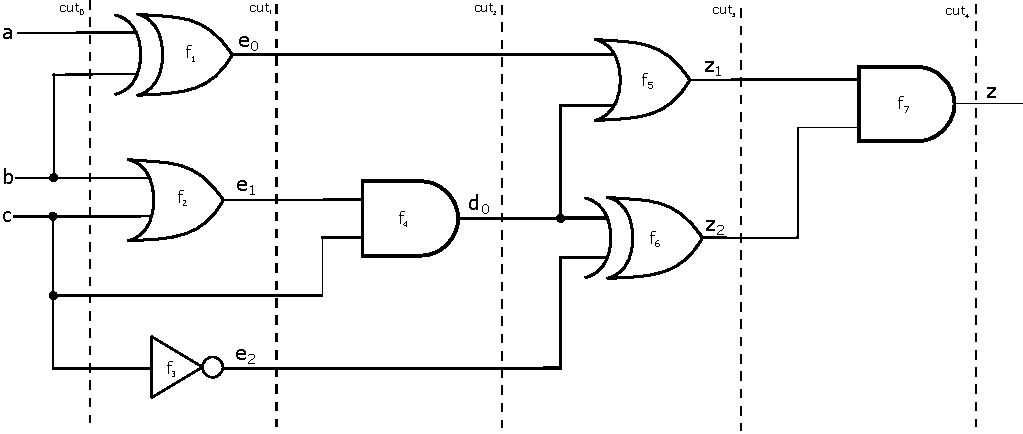
\includegraphics[scale = 0.48]{tianka_ckt_c}
	\end{center}
	\vspace{-1ex}
	\caption{Random logic circuit}
	\label{tianka_ckt_c}
	\vspace{-3.5ex}
\end{figure}

% For the given circuit, we define \textit{cuts} across the gates based on heuristics such as dependency and levelization\cite{maciej:2016:1}. A $cut$ is defined as a set of signals that separates primary inputs from primary outputs. The prominence of these cuts is to maintain a variable order across cuts . For example at each cut $cut_m$ from the figure(\ref{tianka_ckt_c}), the following variable set has to be maintained across reductions.
% \begin{equation}
% \begin{split}
% cut_0 = \{a,b,c\} &\quad cut_3= \{z_1,z_2\}\\
% cut_1 = \{e_0,e_1,c,e_2\}  &\quad cut_4 = \{z\} \\
% cut_2 = \{e_0,d_0,e_2\}
% \end{split}
% \end{equation}
Based on the circuit topology, RTTO$>$ with variable order is given as:
\begin{equation*}
   \{z\}>\{z_1> z_2\}>\{d_0\}>\{e_0> e_1> e_2\}>\{a> b> c\}\\ 
\end{equation*}
Polynomials implementing the given circuit:
\begin{equation}
\begin{split}
 f_1 = e_0 + a + b; &\quad f_5 = z1 + e_0d_0 + e_0 + d_0; \\
 f_2 = e_1 + bc + b + c; &\quad f_6 = z_2 + d_0 + e_2; \\
 f_3 = e_2 + c + 1; &\quad f_7 = z + z_1z_2; \\
 f_4 = d_0 + \mathcal{F}(e_1,c);  
\end{split}
\end{equation}
\begin{equation}
\begin{split}
F = \{f_1,f_2,\dots,f_7\}; & J = \langle F\rangle = \langle f_1,f_2,\dots,f_7\rangle
\end{split}
\end{equation}
We shall add the ideal of vanishing polynomials $J_0$ for primary inputs, outputs, and intermediate variables. 
% Here $\al$ is the root of primitive polynomial used to build the field. 
\begin{align*}
 f_{8}:a^2 + a; &\quad f_{12}:e_1^2 + e_1; &\quad f_{16}:z_2^2 + z_2;\\
 f_{9}:b^2 + b; &\quad f_{13}:e_2^2 + e_2; &\quad f_{17}:z^2 + z;\\
 f_{10}:c^2 + c; &\quad f_{14}:d_0^2 + d_0; \\
 f_{11}:e_0^2 + e_0; &\quad f_{15}:z_1^2 + z_1;
\end{align*}
\begin{equation}
J_0 = \langle f_8,f_9,\dots,f_{17}\rangle
\end{equation}
% Due to RTTO$>$, the set of polynomials ($J+J_0$) is in itself a \Grobner basis.\\
Since the implementation vanishes on specification $f$, we have:
\begin{equation}
f \in \langle f_1,f_2,f_3,f_4,f_5,f_6,f_7\rangle+\langle f_8,f_9,\dots,f_{17}\rangle
\end{equation}
 where tail of $f_4$ is unknown.
% h_4f_4 \in \langle f,f_1,f_2,f_3,f_5,f_6,f_7\rangle\\
% h_4f_4 = f+h_1f_1+h_2f_2+h_3f_3+h_5f_5+h_6f_6+h_7f_7

We know that, under RTTO$>$, the given set of circuit polynomials in itself form a GB. Hence, to compute $g$, we start reducing the specification polynomial $f$ using polynomials from the set $\langle J + J_0\rangle$. We will be using the notations: '[]' to represent quotient-$h_i$'s, '()' to represent divisor-$f_i$'s, and '\{\}' to represent the partial remainder of every reduction step-$fp_i$'s.

\begin{small}
% \begin{split}
$f\quad\xrightarrow[]{f_7}[1](z+z_2z_1)+\{z_2z_1+ac+a+bc+b+c\}\rightarrow fp_1$

$fp_1\quad\xrightarrow[]{f_6}[z_1](z_2+d_0+e_2)+\{z_1d_0+z_1e_2+ac+a+bc+b+c\}\rightarrow fp_2$

$fp_2\quad\xrightarrow[]{f_5}[d_0+e_2](z_1+d_0e_0+d_0+e_0)+\{d_0e_0e_2+d_0e_2+d_0+e_0e_2+ac+a+bc+b+c\}\rightarrow fp_3$

$fp_3\quad\xrightarrow[]{lt(f_4)}[\underbrace{e_0e_2+e_2+1}_\text{$h_4$}](d_0)+ \underbrace{e_0e_2+ac+a+bc+b+c}_\text{g}$

% \end{split}
\end{small}
Reduction order for $f:$
$f\xrightarrow[]{f_7}\xrightarrow[]{f_6}\xrightarrow[]{f_5}\xrightarrow[]{lt(f_4)}g$

% \begin{equation}
% \begin{split}
% h_4f_4+h_1f_1+h_2f_2+h_3f_3 = f+h_5f_5+h_6f_6+h_7f_7;\\
% h_4(d_0+P(e_1,c))+h_1f_1+h_2f_2+h_3f_3 = f+h_5f_5+h_6f_6+h_7f_7;\\
% h_4*d_0+h_4*P(e_1,c)+h_1f_1+h_2f_2+h_3f_3 = f+h_5f_5+h_6f_6+h_7f_7;\\
% h_4*P(e_1,c)+h_1f_1+h_2f_2+h_3f_3 = h_4*d_0+f+h_5f_5+h_6f_6+h_7f_7;\\
% h_4*P(e_1,c)+h_1f_1+h_2f_2+h_3f_3 = e_0*e_2+a*c+a+b*c+b+c;\\
% h_4*P(e_1,c)+h_1f_1+h_2f_2+h_3f_3 = e_0*e_2+a*c+a+b*c+b+c;
% \end{split}
% \end{equation}
Since, we know $h_4,f_1,f_2,f_3$, this can be formulated as ideal membership testing:
\begin{equation*}
\begin{split}
g &\in \langle h_4,f_3,f_2,f_1\rangle + \langle J_0\rangle\\
e_0e_2+ac+a+bc+b+c &\in \langle h_4,f_1,f_2,f_3\rangle + \langle J_0\rangle
\end{split}
\end{equation*}

This ideal membership test can be done using $lift$ procedure in SINGULAR to rewrite a polynomial in terms of an ideal. The procedure takes polynomial $f$ and ideal $J$ in row matrix($[J+J_0]$) as inputs, and returns a column matrix $[U]$ as output such that:
\begin{small}
$f = [U]\cdot [J+J_0]$
\end{small}

% \begin{equation}
% \begin{split}
\begin{small}
$g = \begin{bmatrix} h_4^{'} & h_3^{'} & h_2^{'} & h_1^{'} & \dots & H \end{bmatrix} \cdot 
    \begin{bmatrix} h_4 \\ f_3 \\ f_2 \\ f_1 \\ \vdots \\ x_n^2 + x_n \end{bmatrix}$
\end{small}
% \end{split}
% \end{equation}

\begin{small}
$e_0c+ac+bc+c = [e_0c+ac+bc+c](e_2e_0+e_2+1) + [e_0c+e_0ac+e_0bc+e_0+ac+bc+c](e_2+c+1) + [0](e_1+bc+b+c) + [e_0c+e_0ac+e_0bc+e_0+ac+bc+c](e_0+a+b) + \dots + [0](x_n^2 + x_n)$;
\end{small}

$e_0e_2+ac+a+bc+b+c = [c](e_0e_2+e_2+1) + [e_0c+e_0+c](e_2 + c + 1) + [0](e_1 + bc + b + c) + [c+1](e_0 + a + b);$
\end{Example}

\begin{algorithm}
\caption{Resolve the unknown component for a given circuit}
\label{algo:unknownComponent}
\begin{algorithmic}[1]

\Procedure{$partial\_circuit\_reduction$}{$F,f$}
\State {\it Initialize $h_j\longleftarrow 0$, $r\longleftarrow 0$, $d\longleftarrow f$}
\While{($d\neq 0$)}
\If{$\exists j$ s.t. $lm(f_j)|lm(d)$}
\State {choose $j$ least s.t. $lm(f_j)|lm(d)$}
\State {$h_j = h_j + \frac{lt(d)}{lt(f_j)}$}
\State {$d = d - \frac{lt(d)}{lt(f_j)}f_j$}
\Else
\State {$r = r + lt(d)$}
\State {$d = d - lt(d)$}
\EndIf
\EndWhile
\EndProcedure

\Procedure{$forward\_lifting$}{}

\EndProcedure
\end{algorithmic}
\end{algorithm}

% computing multiple $P$'s:

% we know that:

% $g = Ph_i+h_{i+1}^{'}f_{i+1}+\dots+h_s^{'}f_s+H^{'}\langle x_i^q-x_i\rangle$

% Since $g$ can be computed as any liner combination of polynomials, we can rewrite the equation as:\\
% $Ph_i+h_{i+1}^{'}f_{i+1}+\dots+h_s^{'}f_s+H^{'}\langle x_i^q-x_i\rangle = P^{'}h_i+h_{i+1}^{''}f_{i+1}+\dots+h_s^{''}f_s+H^{''}\langle x_i^q-x_i\rangle$

% rearranging the terms:\\
% $(P-P^{'})h_i = (h_{i+1}^{'}-h_{i+1}^{''})f_{i+1}+\dots+(h_{s}^{'}-h_{s}^{''})f_{s}$

% $(P-P^{'})h_i \in \langle f_{i+1},\dots,f_s\rangle$

% According to definition of Quotient of Ideals:

% $P-P^{'} \in \langle f_{i+1},\dots,f_s\rangle:h_i$

Thus, $P(u_1)=P(e_1,c)=c$, which can implemented as a simple AND gate with $c$ as both inputs. 

Since any $P_i$ which satisfies $P_i-P_j\in(f_1,f_2,f_3):h_4$, where $i\neq j$, works for the circuit, the computed $P$ is not considered unique and can take any values. We need to come up with better heuristics to identify the exact form and variables in which we want the $P$ to be. 


% \begin{figure}[ht]
% 	\begin{center}
% 	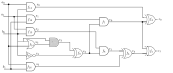
\includegraphics[scale = 0.40]{mas_c}
% 	\end{center}
% 	\vspace{-1ex}
% 	\caption{correct implementation mastrovito}
% 	\label{mas_c}
% 	\vspace{-1ex}
% \end{figure}

% \begin{figure}[ht]
% 	\begin{center}
% 	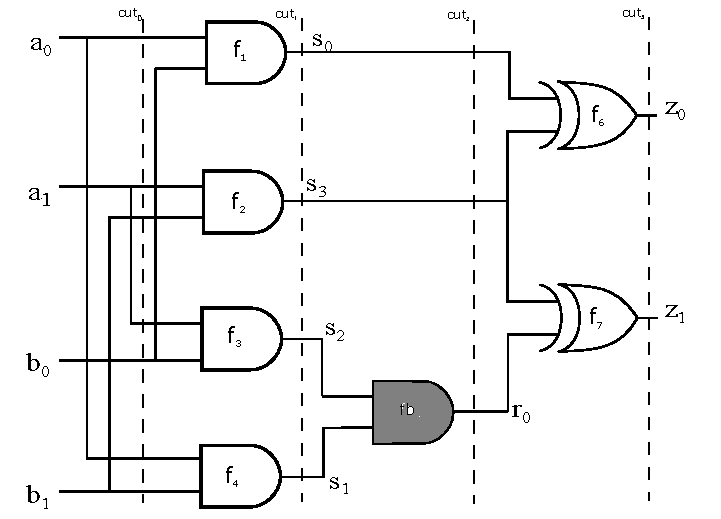
\includegraphics[scale = 0.40]{mas_b}
% 	\end{center}
% 	\vspace{-4ex}
% 	\caption{buggy implementation mastrovito}
% 	\label{mas_b}
% 	\vspace{-2ex}
% \end{figure}